\section{Completamento: Simulink linearizzato e RAS LQRI}
\label{sec:simulink-completion}
Le verifiche seguenti estendono l'integrazione senza ricostruire i quattro
modelli non lineari, modificare controllori o rieseguire sintesi e analisi robuste.
Sono eseguite con MATLAB/Simulink R2025b Update 4.

\subsection{Un solo diagramma lineare per quattro controllori}
Il modello \path{simulink/models/SEA_linear_common.slx} contiene esplicitamente
il plant completo M3, realizzato con un blocco State-Space di 14 stati:
\[
 \dot x=A_{\rm full}x+[B_{\rm full}\ B_{d,\rm full}]
 \begin{bmatrix}u\\d\end{bmatrix},\quad
 y=C_{\rm full,Meas}x,\qquad q=C_{\rm full,Q}x.
\]
Gli ultimi due prodotti sono blocchi Gain distinti: quattro misure e due
posizioni dei link. I primi otto stati sono meccanici, gli ultimi sei degli
attuatori. Tutte le coordinate del diagramma lineare sono incrementali;
lo zero corrisponde all'equilibrio assoluto del modello non lineare.
Il disturbo entra tramite $B_{d,\rm full}$, senza attraversare gli attuatori.

\path{setup_linear_common.m} seleziona le matrici del controllore dagli
stessi artifact dell'integrazione. LQG e LQRI ricevono $[r;y]$ (sei ingressi);
H-infinity e Kmu ricevono $[r;q]$ (quattro ingressi), conservando la vera
architettura 2-DoF a stati condivisi. Il selettore riguarda solo le misure
al controllore, non elimina stati dalla pianta. Gli ordini complessivi sono
28, 30, 36 e 92; non si applicano riduzioni o \texttt{minreal}.
Per LQG lo stato interno iniziale è $\hat x_0$, per LQRI è
$[\hat x_0;\xi_0]$. Il plant comune è deterministico: la validazione dei
rumori resta nei quattro modelli non lineari già verificati.

\subsection{Due confronti distinti, con esiti numerici}
Per ogni controllore si eseguono tre simulazioni lineari di 3 s:
gradino di $5^\circ$ sul primo giunto, sul secondo giunto e, a riferimento
nullo, disturbo $[0.01;-0.007]$ N m sui link da $t=0$.
La mappa MATLAB indipendente è assemblata da plant e controllore e simulata
con \texttt{lsim}; non è una linearizzazione automatica del nuovo diagramma.
Il solver del modello lineare è \texttt{ode23t}, con tolleranze relativa
$10^{-9}$, assoluta $10^{-11}$ e passo massimo 0.002 s.
Le uscite sono confrontate sulla griglia 0.002 s, interpolando linearmente
i campioni del solver. Le differenze includono dunque errore numerico e
di interpolazione, non una discrepanza di progetto.

Si esegue inoltre il modello lineare con $r=[10^{-4};-7\,10^{-5}]$ rad
per 3 s e lo si confronta con le tracce non lineari già validate e conservate
in \path{results/data/simulink_integration/*_runs.mat}.
Riutilizzare queste tracce evita di ripetere la campagna precedente;
le matrici e i modelli sorgente restano invariati.
\begin{table}[htbp]\centering\small
\begin{tabular}{lrrrr}\toprule
 & \multicolumn{2}{c}{Lineare SL / MATLAB} & \multicolumn{2}{c}{Non lineare SL / lineare SL}\\
 & max $|e_q|$ [rad] & max $|e_u|$ [Nm] & max $|e_q|$ [rad] & max $|e_u|$ [Nm]\\\midrule
LQG & 6.095e-09 & 5.141e-07 & 7.261e-10 & 1.495e-07 \\
LQRI & 1.072e-08 & 9.062e-08 & 2.895e-10 & 3.644e-08 \\
Hinf & 3.301e-09 & 1.792e-06 & 8.420e-10 & 4.615e-08 \\
Kmu & 1.573e-09 & 1.413e-08 & 9.800e-10 & 1.147e-08 \\
\bottomrule\end{tabular}
\caption{Massimi sui tre scenari per le prime due colonne; piccolo segnale
per le ultime due. SL indica Simulink. Dati: linear\_summary.json.}
\end{table}
Tutte le 32 verifiche numeriche superano le soglie, fissate prima del calcolo,
di $2\,10^{-7}$ rad e $2\,10^{-4}$ N m, coerenti con l'integrazione precedente.
Queste soglie verificano l'equivalenza implementativa, non i target M5.
\begin{figure}[htbp]\centering
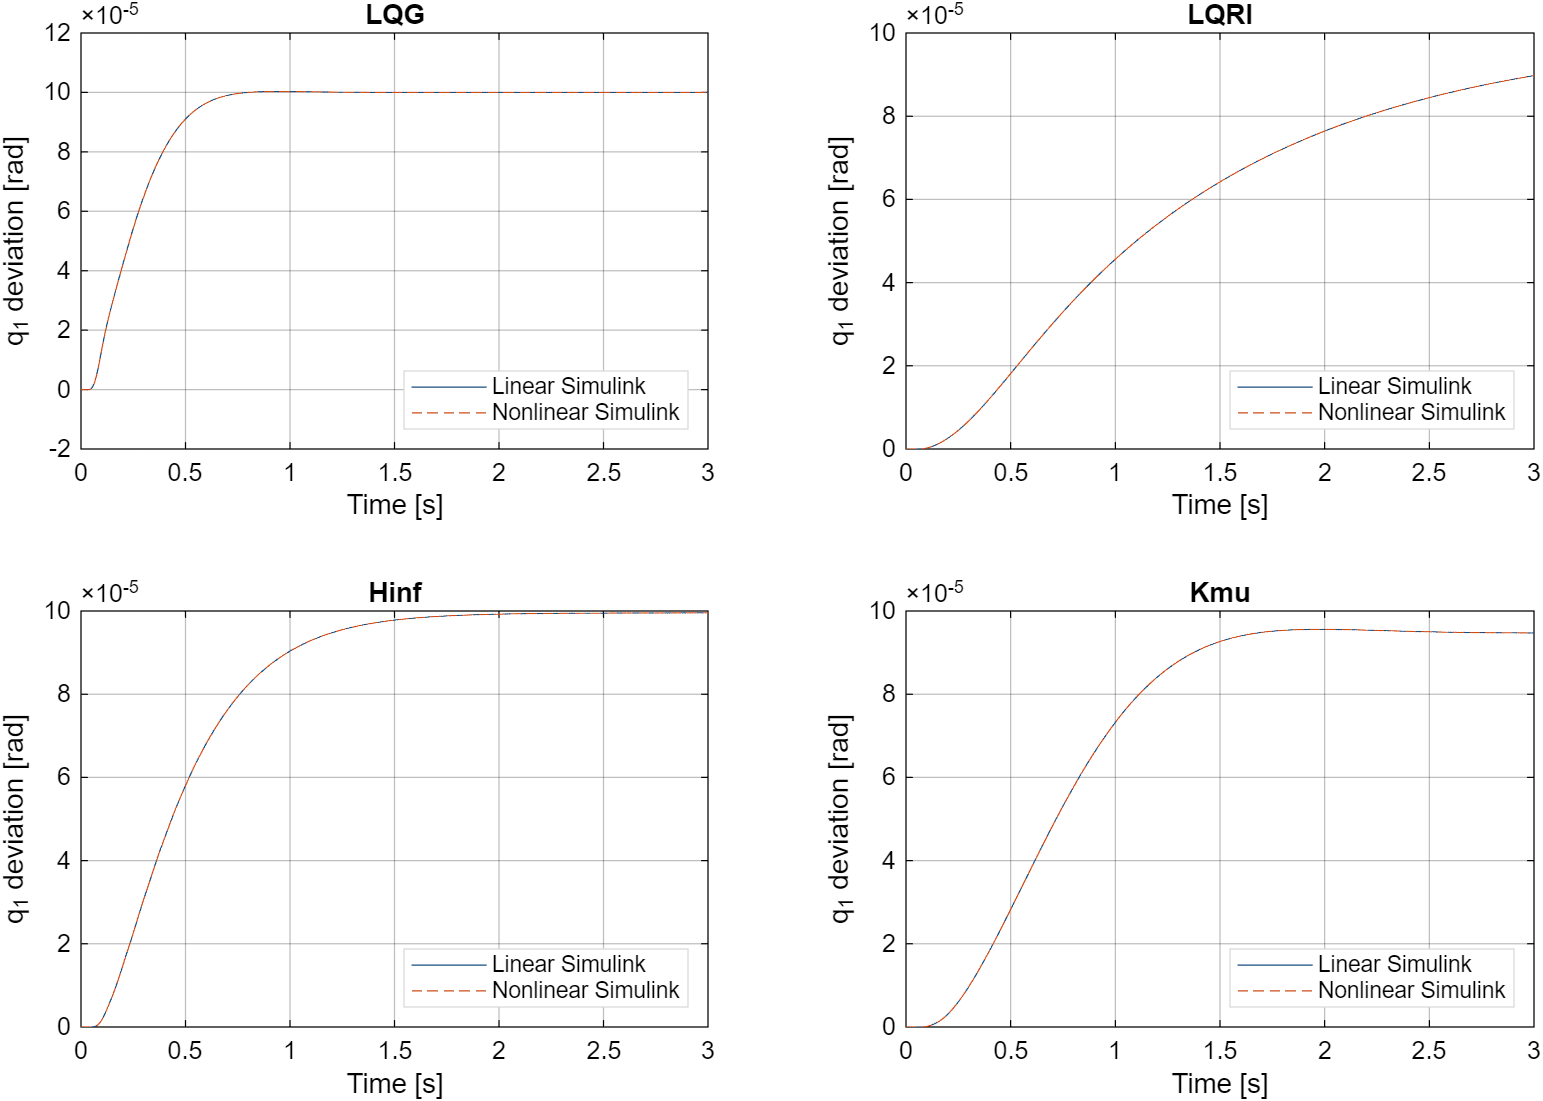
\includegraphics[width=.90\textwidth]{figures/simulink_completion/linear_nonlinear.png}
\caption{Sovrapposizione delle traiettorie lineari e non lineari a piccolo segnale.}
\end{figure}

\subsection{RAS nominale LQRI: stesso protocollo, stessi limiti interpretativi}
La ricerca utilizza direttamente \path{estimate_lqg_ras.m} e
\path{evaluate_m8_convergence.m}. Alla funzione di ricerca sono aggiunti
solo un simulatore opzionale e un checkpoint: le chiamate storiche M8
mantengono i valori predefiniti. L'adattatore esegue
\texttt{SEA\_LQRI\_integrated}, senza cambiare $K_x,K_i,L,Q_n,R_n$.
Il confronto LQG usa i dati M8 salvati: un test verifica l'identità esatta
dei guadagni $K,L,N_r$ rispetto agli artifact correnti.

La sezione iniziale è
$\delta x_{\rm mech}=[\delta q;0_2;\delta q;0_2]$,
con attuatori all'equilibrio, $\hat x_0=0_{14}$ e, per LQRI, $\xi_0=0_2$.
Riferimento, disturbo e rumori sono nulli; non sono introdotte saturazioni.
Si usa il box $[-60,60]^2$ gradi, griglia iniziale $5\times5$, 36 direzioni
a intervalli di $10^\circ$ e bisezione radiale con precisione $1^\circ$
se l'estremo non converge. Il budget massimo è 400 simulazioni.
Il solver è \texttt{ode23t}, tolleranze $10^{-5}$ e $10^{-7}$,
passo massimo 0.005 s: gli stessi valori di M8.

L'orizzonte è 8 s, estendibile a 12 s secondo il criterio M8.
La coda è l'ultimo 10\% dei \emph{campioni del solver}, come nel codice storico:
non è una nuova griglia uniforme né necessariamente l'ultimo 10\% del tempo.
Le soglie sono $0.5^\circ$ per link e rotori, 0.02 rad/s per i link e
0.05 rad/s per i rotori, con controllo della crescita finale
(fattore 0.05 e pavimento $0.05^\circ$). Le traiettorie devono essere
complete, finite e limitate a $10^6$; si controlla anche lo stato integrale.
La sezione opzionale con stima iniziale coerente non è rieseguita per LQRI.

\begin{table}[htbp]\centering
\begin{tabular}{lrr}\toprule
Protocollo nominale, stima iniziale nulla & LQG M6 & LQRI M7\\\midrule
Punti convergenti / esaminati & 57/57 & 57/57\\
Simulazioni / estensioni a 12 s & 57 / 0 & 57 / 0\\
Raggio minimo risolto [gradi] & 60 & 60\\
Raggio massimo campionato [gradi] & 78.3244 & 78.3244\\
Area del poligono campionato [gradi$^2$] & 14213.60 & 14213.60\\
Massimo comando osservato [Nm] & 232.1879 & 240.9605\\\bottomrule
\end{tabular}
\caption{Entrambe le ricerche sono SEARCH-BOX LIMITED e non certificate.}
\end{table}
Non si osservano errori di simulazione, punti non convergenti o necessità
di estendere l'orizzonte LQRI. Il risultato non stabilisce quale controllore
abbia la RAS effettiva maggiore: entrambe le ricerche raggiungono il bordo.
Il raggio massimo supera $60^\circ$ perché è una distanza radiale in un box.
L'area è quella del poligono delle direzioni campionate; non è una misura
certificata della RAS. La ricerca finita non esclude punti interni sfavorevoli
o regioni non connesse radialmente. I picchi superiori a 200 Nm non sono
confrontati con un limite hardware non identificato.
\begin{figure}[htbp]\centering
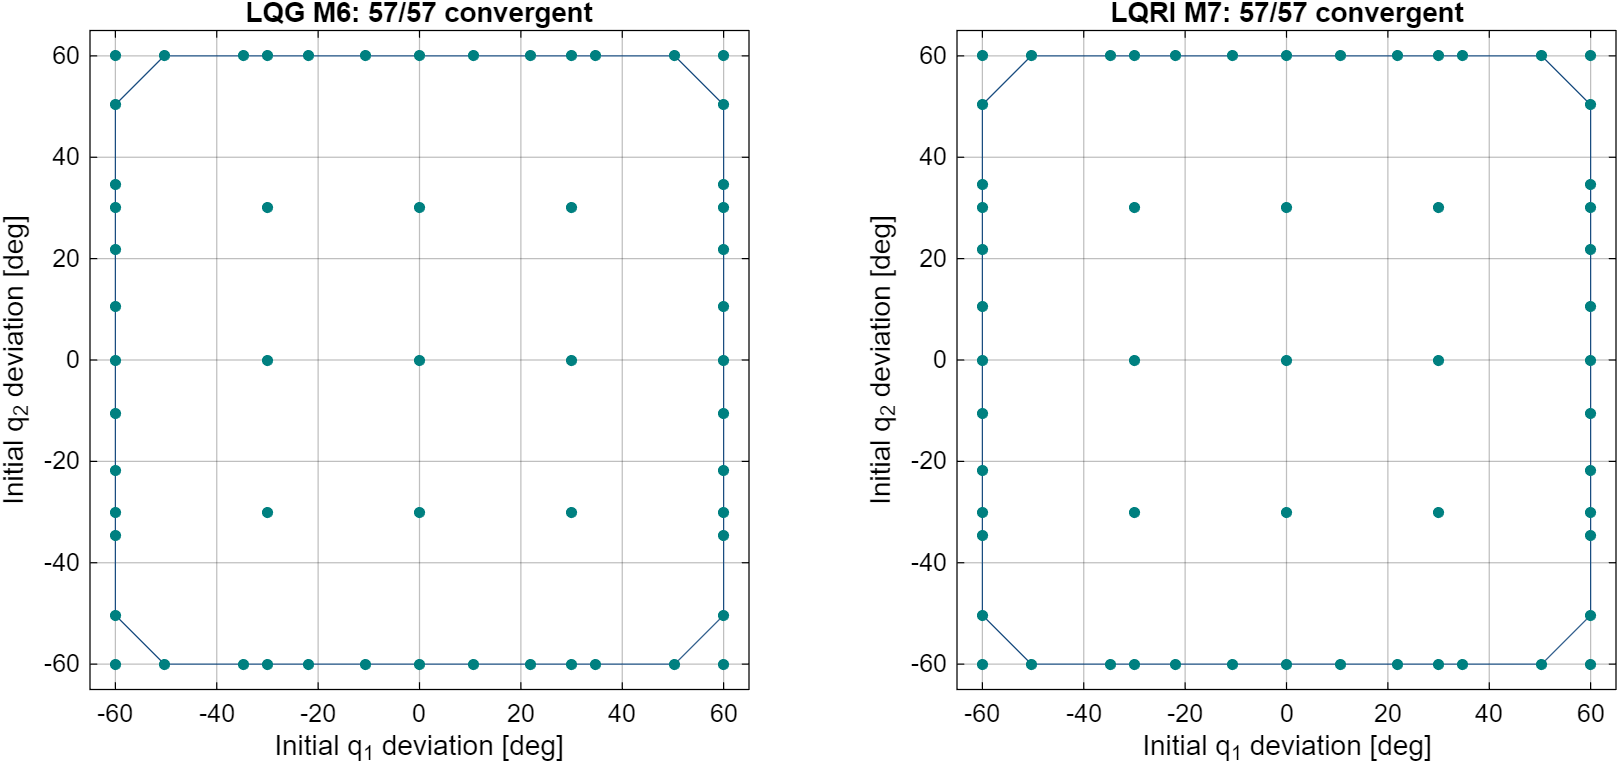
\includegraphics[width=\textwidth]{figures/simulink_completion/ras_lqg_lqri.png}
\caption{Sezioni empiriche LQG e LQRI nel medesimo dominio. La frontiera
del disegno è il limite della ricerca, non una frontiera di stabilità provata.}
\end{figure}

\subsection{Test aggiunti e tracciabilità degli errori di sviluppo}
Restano intatti i 67 controlli e i sette test precedenti. La nuova suite
aggiunge 15 casi: quattro confronti lineari, quattro confronti a piccolo
segnale, quattro verifiche del diagramma M3 e degli ordini totali, tre
verifiche del protocollo RAS, dell'assenza di errori e dell'identità LQG.
I sette test originari sono rieseguiti insieme ai nuovi: 22/22 PASS.
Le 67 simulazioni di verifica originarie non sono rilanciate;
la loro evidenza salvata resta 67/67 PASS e viene controllata dalla suite.

Il primo run dei test ha prodotto quattro FAIL per un errore nel test:
\texttt{linmod} con un solo output restituisce una struttura, non la matrice A.
La chiamata è stata corretta richiedendo quattro output; modello e soglie
non sono cambiati. MAT e CSV del run iniziale sono conservati con suffisso
\texttt{initial\_failure}. Le simulazioni numeriche non avevano fallito.
Il nuovo percorso \texttt{CR\_RUN\_SCOPE=simulink-completion} rigenera solo
modello lineare, confronti e RAS nominale (ripresa da checkpoint compatibile).
Le evidenze sono in \path{results/data/simulink_completion}; nessun risultato
robusto precedente è ricalcolato o sostituito.
